\chapter{模式相关物理常数/参数}\label{模式相关物理常数参数}
%\addcontentsline{toc}{chapter}{附录}
%\begin{附录}
%\section{附录 A: 模式相关物理常数/参数}
% Please add the following required packages to your document preamble:
% \usepackage{booktabs}
\begin{table}[htbp]
    \centering
    \caption{物理常数}
    \label{tab:物理常数}
    \begin{tabular}{@{}lc@{}}
    \toprule
    名称 {[}单位{]}                                     & 常数值       \\
    \midrule
    固态水密度 {[}\unit{kg.m^{-3}}{]}                  & 917.0        \\
    液态水密度 {[}\unit{kg.m^{-3}}{]}                  & 1000.0       \\
    液态水比热容 {[}\unit{J.kg^{-1}.K^{-1}}{]}         & 4188.0       \\
    固态水比热容 {[}\unit{J.kg^{-1}.K^{-1}}{]}         & 2117.27     \\
    干空气比热容 {[}\unit{J.kg^{-1}.K.^{-1}}{]}        & 1004.64     \\
    固态水液化潜热 {[}\unit{J.kg^{-1}}{]}             & \num{0.3336e6}  \\
    液态水蒸发潜热 {[}\unit{J.kg^{-1}}{]}             & \num{2.5104e6}  \\
    固态水升华潜热 {[}\unit{J.kg^{-1}}{]}             & \num{2.8440e6}  \\
    空气热力传导率 {[}\unit{W.m^{-1}.K^{-1}}{]}       & 0.023       \\
    固态水热力传导率 {[}\unit{W.m^{-1}.K^{-1}}{]}      & 2.290       \\
    液态水热力传导率 {[}\unit{W.m^{-1}.K^{-1}}{]}      & 0.6         \\
    液态水凝结温度 {[}K{]}                             & 273.16      \\
    干空气气体常数 {[}\unit{J.kg^{-1}.K^{-1}}{]}       & 287.04      \\
    rw/g = (8.3144/0.018)/(9.80616)*1000. {[}\unit{mm.K^{-1}}{]} & \num{4.71047e4} \\
    水汽气体常数{[}\unit{J.kg^{-1}.K^{-1}}{]}         & 461.296     \\
    重力加速度 {[}\unit{m.s^{-2}}{]}                  & 9.80616     \\
    von K\'arman常数 {[}-{]}                         & 0.4         \\
    Stefan-Boltzmann常数 {[}\unit{W.m^{-2}.K^{-4}}{]} & \num{5.67e-8}\\
    \bottomrule
    \end{tabular}
\end{table}

% Please add the following required packages to your document preamble:
% \usepackage{booktabs}
\begin{table}[htbp]
\centering
\caption{其他全局参数设定值。}
\label{tab:其他全局参数设定值}
\begin{tabular}{@{}lc@{}}
\toprule
名称 {[}单位{]}                               & 参数值      \\
\midrule
土壤粗糙度 {[}m{]}                             & 0.01     \\
积雪覆盖地表粗糙度 {[}m{]}                         & 0.0024   \\
林下冠层与土壤热力/水汽交换系数 {[}-{]}                  & 0.004    \\
叶片最大载水量 {[}mm{]}                          & 0.1      \\
表层土壤水饱和区最大覆盖比例 (Niu et al., 2005) {[}-{]} & 0.38     \\
表层温度到表面温度转换系数 {[}-{]}                     & 0.34     \\
Crank Nicholson隐式格式权重因子 {[}-{]}           & 0.5      \\
积雪孔隙中的最大液态水饱和度 {[}-{]}                    & 0.033    \\
土壤可透水最小孔隙度 {[}-{]}                        & 0.05     \\
地面最大积水深度 {[}mm{]}                         & 10.0     \\
萎焉点土壤水势 {[}mm{]}                          & \num{-1.5e5} \\
最小土壤水势 {[}mm{]}                           & \num{-1e8}   \\
最大蒸腾速率 [\unit{mm.s^{-1}}]                 & \num{2e-4}   \\
确定雨/雪临界温度 {[}\textcelsius {]}            & 2.5      \\
\bottomrule
\end{tabular}
\end{table}


\chapter{USGS地表覆盖类型相关参数}\label{USGS地表覆盖类型相关参数}

% Please add the following required packages to your document preamble:
% \usepackage{booktabs}
\begin{table}[htbp]
    \centering
    \caption{USGS地表覆盖植被顶部高度和底部高度值(当无植被高度数据读入时的默认高度)。}
    \label{tab:USGS地表覆盖植被顶部高度和底部高度值}
    \begin{tabular}{@{}lcc@{}}
    \toprule
    USGS地表覆盖类型     & 植被顶部高度 (m) & 植被底部高度 (m) \\ \midrule
    1 城市           & 1          & 0          \\
    2 干旱农田与牧场      & 0.5        & 0          \\
    3 灌溉农田与牧场      & 0.5        & 0          \\
    4 干旱/灌溉混合农田与牧场 & 0.5        & 0          \\
    5 农田草地过渡带      & 0.5        & 0          \\
    6 农田林地过渡带      & 0.5        & 0          \\
    7 草地           & 0.5        & 0          \\
    8 灌木地          & 0.5        & 0          \\
    9 草地灌木地混合带     & 0.5        & 0          \\
    10 稀疏草原        & 0.5        & 0          \\
    11 落叶阔叶林       & 20         & 1          \\
    12 落叶针叶林       & 17         & 1          \\
    13 常绿阔叶林       & 35         & 1          \\
    14 常绿针叶林       & 17         & 1          \\
    15 混合森林        & 20         & 1          \\
    16 内陆水体        & 0.5        & 0          \\
    17 草本湿地        & 0.5        & 0          \\
    18 森林湿地        & 17         & 1          \\
    19 贫瘠稀疏植被      & 0.5        & 0          \\
    20 草本苔原        & 0.5        & 0          \\
    21 森林苔原        & 0.5        & 0          \\
    22 混合苔原        & 0.5        & 0          \\
    23 裸土苔原        & 0.5        & 0          \\
    24 雪盖或冰川       & 0.5        & 0          \\ \bottomrule
    \end{tabular}
\end{table}

% Please add the following required packages to your document preamble:
% \usepackage{booktabs}
\begin{table}[htbp]
\centering
\caption{USGS地表覆盖植被茎面积指数(当无植被茎面积指数数据读入时的默认值)。}
\label{tab:USGS地表覆盖植被茎面积指数}
\begin{tabular}{@{}lc@{}}
\toprule
USGS地表覆盖类型     & 茎面积指数 (\unit{m^2.m^{-2}}) \\ \midrule
1 城市           & 0.2       \\
2 干旱农田与牧场      & 0.2       \\
3 灌溉农田与牧场      & 0.3       \\
4 干旱/灌溉混合农田与牧场 & 0.3       \\
5 农田草地过渡带      & 0.5       \\
6 农田林地过渡带      & 0.5       \\
7 草地           & 1         \\
8 灌木地          & 0.5       \\
9 草地灌木地混合带     & 1         \\
10 稀疏草原        & 0.5       \\
11 落叶阔叶林       & 2         \\
12 落叶针叶林       & 2         \\
13 常绿阔叶林       & 2         \\
14 常绿针叶林       & 2         \\
15 混合森林        & 2         \\
16 内陆水体        & 0         \\
17 草本湿地        & 0.2       \\
18 森林湿地        & 2         \\
19 贫瘠稀疏植被      & 0.2       \\
20 草本苔原        & 0.2       \\
21 森林苔原        & 0.2       \\
22 混合苔原        & 0.2       \\
23 裸土苔原        & 0         \\
24 雪盖或冰川       & 0         \\\bottomrule
\end{tabular}
\end{table}

% Please add the following required packages to your document preamble:
% \usepackage{booktabs}
\begin{table}[htbp]
\centering
\caption{USGS地表覆盖粗糙度及零平面位移与植被高度比值(为CoLM2014默认方案,目前版本使用公式 \eqref{dOh}, \eqref{zOh} 和 \eqref{dooh})。}
\label{tab:USGS地表覆盖粗糙度及零平面位移与植被高度比值}
\begin{tabular}{@{}lcc@{}}
\toprule
USGS地表覆盖类型     & 粗糙度与植被高度比值 & 零平面位移与植被高度比值 \\ \midrule
1 城市           & 0.1        & 0.667        \\
2 干旱农田与牧场      & 0.1        & 0.667        \\
3 灌溉农田与牧场      & 0.1        & 0.667        \\
4 干旱/灌溉混合农田与牧场 & 0.1        & 0.667        \\
5 农田草地过渡带      & 0.1        & 0.667        \\
6 农田林地过渡带      & 0.1        & 0.667        \\
7 草地           & 0.1        & 0.667        \\
8 灌木地          & 0.1        & 0.667        \\
9 草地灌木地混合带     & 0.1        & 0.667        \\
10 稀疏草原        & 0.1        & 0.667        \\
11 落叶阔叶林       & 0.1        & 0.667        \\
12 落叶针叶林       & 0.1        & 0.667        \\
13 常绿阔叶林       & 0.1        & 0.667        \\
14 常绿针叶林       & 0.1        & 0.667        \\
15 混合森林        & 0.1        & 0.667        \\
16 内陆水体        & 0.1        & 0.667        \\
17 草本湿地        & 0.1        & 0.667        \\
18 森林湿地        & 0.1        & 0.667        \\
19 贫瘠稀疏植被      & 0.1        & 0.667        \\
20 草本苔原        & 0.1        & 0.667        \\
21 森林苔原        & 0.1        & 0.667        \\
22 混合苔原        & 0.1        & 0.667        \\
23 裸土苔原        & 0.1        & 0.667        \\
24 雪盖或冰川       & 0.1        & 0.667        \\ \bottomrule
\end{tabular}
\end{table}


% Please add the following required packages to your document preamble:
% \usepackage{booktabs}
\begin{landscape}
\begin{table}[htbp]
%\begin{sidewaystable}[]
\centering
\caption{USGS植被特征尺寸、叶倾角分布及叶片光学属性参数。$\chi_L$为叶倾角分布参数,$\rho$表示反射率,$\tau$表示透射率,下标$l$表示叶片,$s$表示茎,$vis$表示可见光波段,$nir$表示近红外波段。}
\label{tab:USGS植被特征尺寸叶倾角分布及叶片光学属性参数1}
    \begin{tabular}{@{}lcccccccccc@{}}
    \toprule
    USGS地表覆盖类型     & 叶片特征尺寸(cm) & $\chi_L$ &$\rho_{l, vis}$ & $\tau_{l, vis}$  &$\rho_{l, nir}$ &$\tau_{l, nir}$ & $\rho_{s, vis}$ &$\tau_{s, vis}$ &$\rho_{s, nir}$ &$\tau_{s,nir}$\\ \midrule
    1 城市           & 4.0        & \num{ -0.3  }                                                                       & 0.105                                                                                                           & 0.07                                                                                                            & 0.58                                                                                                            & 0.25                                                                                                            & 0.36                                                                                                            & 0.22                                                                                                            & 0.58                                                                                                            & 0.38                                                                                                            \\
    2 干旱农田与牧场      & 4.0        & \num{ -0.3  }                                                                       & 0.105                                                                                                           & 0.07                                                                                                            & 0.58                                                                                                            & 0.25                                                                                                            & 0.36                                                                                                            & 0.22                                                                                                            & 0.58                                                                                                            & 0.38                                                                                                            \\
    3 灌溉农田与牧场      & 4.0        & \num{ -0.3  }                                                                       & 0.105                                                                                                           & 0.07                                                                                                            & 0.58                                                                                                            & 0.25                                                                                                            & 0.36                                                                                                            & 0.22                                                                                                            & 0.58                                                                                                            & 0.38                                                                                                            \\
    4 干旱/灌溉混合农田与牧场 & 4.0        & \num{ -0.3  }                                                                       & 0.105                                                                                                           & 0.07                                                                                                            & 0.58                                                                                                            & 0.25                                                                                                            & 0.36                                                                                                            & 0.22                                                                                                            & 0.58                                                                                                            & 0.38                                                                                                            \\
    5 农田草地过渡带      & 4.0        & \num{ -0.3  }                                                                       & 0.105                                                                                                           & 0.07                                                                                                            & 0.58                                                                                                            & 0.25                                                                                                            & 0.36                                                                                                            & 0.22                                                                                                            & 0.58                                                                                                            & 0.38                                                                                                            \\
    6 农田林地过渡带      & 4.0        & \num{ -0.3  }                                                                       & 0.105                                                                                                           & 0.07                                                                                                            & 0.58                                                                                                            & 0.25                                                                                                            & 0.36                                                                                                            & 0.22                                                                                                            & 0.58                                                                                                            & 0.38                                                                                                            \\
    7 草地           & 4.0        & \num{ -0.3  }                                                                       & 0.105                                                                                                           & 0.07                                                                                                            & 0.58                                                                                                            & 0.25                                                                                                            & 0.36                                                                                                            & 0.22                                                                                                            & 0.58                                                                                                            & 0.38                                                                                                            \\
    8 灌木地          & 4.0        & \num{ 0.01  }                                                                       & 0.1                                                                                                             & 0.07                                                                                                            & 0.45                                                                                                            & 0.25                                                                                                            & 0.16                                                                                                            & 0.001                                                                                                           & 0.39                                                                                                            & 0.001                                                                                                           \\
    9 草地灌木地混合带     & 4.0        & \num{ 0.01  }                                                                       & 0.1                                                                                                             & 0.07                                                                                                            & 0.45                                                                                                            & 0.25                                                                                                            & 0.16                                                                                                            & 0.001                                                                                                           & 0.39                                                                                                            & 0.001                                                                                                           \\
    10 稀疏草原        & 4.0        & \num{ -0.3  }                                                                       & 0.105                                                                                                           & 0.07                                                                                                            & 0.58                                                                                                            & 0.25                                                                                                            & 0.36                                                                                                            & 0.22                                                                                                            & 0.58                                                                                                            & 0.38                                                                                                            \\
    11 落叶阔叶林       & 4.0        & \num{ 0.25  }                                                                       & 0.1                                                                                                             & 0.05                                                                                                            & 0.45                                                                                                            & 0.25                                                                                                            & 0.16                                                                                                            & 0.001                                                                                                           & 0.39                                                                                                            & 0.001                                                                                                           \\
    12 落叶针叶林       & 4.0        & \num{ 0.01  }                                                                       & 0.07                                                                                                            & 0.05                                                                                                            & 0.35                                                                                                            & 0.1                                                                                                             & 0.16                                                                                                            & 0.001                                                                                                           & 0.39                                                                                                            & 0.001                                                                                                           \\ %\bottomrule
%    \end{tabular}
%\end{sidewaystable}
%
%% Please add the following required packages to your document preamble:
%% \usepackage{booktabs}
%\begin{sidewaystable}[]
%    \centering
%    \caption{USGS植被特征尺寸、叶倾角分布及叶片光学属性参数 (续)。$\chi_L$为叶倾角分布参数,$\rho$表示反射率,$\tau$表示透射率,下标$l$表示叶片,$s$表示茎,$vis$表示可见光波段,$nir$表示近红外波段。}
%    \label{tab:USGS植被特征尺寸叶倾角分布及叶片光学属性参数2}
%        \begin{tabular}{@{}lcccccccccc@{}}
%        \toprule
%        USGS地表覆盖类型     & 叶片特征尺寸(cm) & $\chi_L$ &$\rho_{l, vis}$ & $\tau_{l, vis}$  &$\rho_{l, nir}$ &$\tau_{l, nir}$ & $\rho_{s, vis}$ &$\tau_{s, vis}$ &$\rho_{s, nir}$ &$\tau_{s, nir}$\\ \midrule
        13 常绿阔叶林   & 4.0        & \num { 0.1   }                                                                       & 0.1                                                                                                             & 0.05                                                                                                            & 0.45                                                                                                            & 0.25                                                                                                            & 0.16                                                                                                            & 0.001                                                                                                           & 0.39                                                                                                            & 0.001                                                                                                           \\
        14 常绿针叶林   & 4.0        & \num { 0.01  }                                                                       & 0.07                                                                                                            & 0.05                                                                                                            & 0.35                                                                                                            & 0.1                                                                                                             & 0.16                                                                                                            & 0.001                                                                                                           & 0.39                                                                                                            & 0.001                                                                                                           \\
        15 混合森林    & 4.0        & \num { 0.125 }                                                                       & 0.07                                                                                                            & 0.05                                                                                                            & 0.4                                                                                                             & 0.15                                                                                                            & 0.16                                                                                                            & 0.001                                                                                                           & 0.39                                                                                                            & 0.001                                                                                                           \\
        16 内陆水体    & 4.0        & \num { -0.3  }                                                                       & 0.105                                                                                                           & 0.07                                                                                                            & 0.58                                                                                                            & 0.25                                                                                                            & 0.36                                                                                                            & 0.22                                                                                                            & 0.58                                                                                                            & 0.38                                                                                                            \\
        17 草本湿地    & 4.0        & \num { -0.3  }                                                                       & 0.1                                                                                                             & 0.07                                                                                                            & 0.58                                                                                                            & 0.25                                                                                                            & 0.36                                                                                                            & 0.22                                                                                                            & 0.58                                                                                                            & 0.38                                                                                                            \\
        18 森林湿地    & 4.0        & \num { 0.1   }                                                                       & 0.105                                                                                                           & 0.05                                                                                                            & 0.45                                                                                                            & 0.25                                                                                                            & 0.16                                                                                                            & 0.001                                                                                                           & 0.39                                                                                                            & 0.001                                                                                                           \\
        19 贫瘠稀疏植被  & 4.0        & \num { 0.01  }                                                                       & 0.1                                                                                                             & 0.07                                                                                                            & 0.45                                                                                                            & 0.25                                                                                                            & 0.16                                                                                                            & 0.001                                                                                                           & 0.39                                                                                                            & 0.001                                                                                                           \\
        20 草本苔原    & 4.0        & \num { -0.3  }                                                                       & 0.07                                                                                                            & 0.07                                                                                                            & 0.58                                                                                                            & 0.25                                                                                                            & 0.36                                                                                                            & 0.22                                                                                                            & 0.58                                                                                                            & 0.38                                                                                                            \\
        21 森林苔原    & 4.0        & \num { -0.3  }                                                                       & 0.1                                                                                                             & 0.07                                                                                                            & 0.58                                                                                                            & 0.25                                                                                                            & 0.36                                                                                                            & 0.22                                                                                                            & 0.58                                                                                                            & 0.38                                                                                                            \\
        22 混合苔原    & 4.0        & \num { -0.3  }                                                                       & 0.07                                                                                                            & 0.07                                                                                                            & 0.58                                                                                                            & 0.25                                                                                                            & 0.36                                                                                                            & 0.22                                                                                                            & 0.58                                                                                                            & 0.38                                                                                                            \\
        23 裸土苔原    & 4.0        & \num { -0.3  }                                                                       & 0.07                                                                                                            & 0.07                                                                                                            & 0.58                                                                                                            & 0.25                                                                                                            & 0.36                                                                                                            & 0.22                                                                                                            & 0.58                                                                                                            & 0.38                                                                                                            \\
        24 雪盖或冰川   & 4.0        & \num { -0.3  }                                                                       & 0.105                                                                                                           & 0.07                                                                                                            & 0.58                                                                                                            & 0.25                                                                                                            & 0.36                                                                                                            & 0.22                                                                                                            & 0.58                                                                                                            & 0.38                                                                                                            \\\bottomrule
                \end{tabular}
%\end{sidewaystable}
\end{table}
\end{landscape}


% Please add the following required packages to your document preamble:
% \usepackage{booktabs}
\begin{landscape}
\begin{table}[htbp]
%\begin{sidewaystable}[]
    \centering
    \caption{USGS植被光合作用参数。$V_{cmax}$表示植被冠层顶部 25~\textcelsius 时光合最大羧化速率(\unit{mol.m^{-2}.s^{-1}}),$\alpha$为量子转化效率(0.05 \unit{mol.CO_2.mol^{-1}.photon}),$m$为气孔导度经验拟合经验参数(无量纲),$b$为最小气孔导度(\unit{mol.CO_2.m^{-2}.s^{-1}}) ,
    $r_{base}$为叶基础呼吸速率系数(无量纲),$s_1$是高温抑制系数(\unit{K^{-1}}),$s_2$是低温抑制系数(\unit{K^{-1}}),$s_3$是叶呼吸高温抑制系数(\unit{K^{-1}}),$T_{dm}$是叶呼吸高温抑制温度参数(K)。}
    \label{tab:USGS植被光合作用参数1}
    \begin{tabular}{@{}lccccccccccccccccccc@{}}
    \toprule
    USGS地表覆盖类型     &$ V_{cmax}$ & $\alpha$ & $m$& $b$ & $r_{base}$ & $s_1$ & $s_2$ & $s_3$ & $T_{dm}$ & $T_{op}$ & $T_{low}$ & $T_{high}$ & $K_n$  \\ \midrule
    1 城市     & 100  & 0.08  & 9  & 0.01  & 0.015  & 0.3 & 0.2 & 1.3  & 328  & 298  & 308  & 281  & 0.5 \\
    2 干旱农田与牧场      & 57  & 0.08  & 9  & 0.01   & 0.015 & 0.3  & 0.2  & 1.3  & 328   & 298  & 308  & 281  & 0.5  \\
    3 灌溉农田与牧场      & 57  & 0.08  & 9  & 0.01   & 0.015 & 0.3  & 0.2 & 1.3   & 328   & 298  & 308 & 281   & 0.5  \\
    4 干旱/灌溉混合农田与牧场 & 57  & 0.08  & 9  & 0.01  & 0.015  & 0.3  & 0.2  & 1.3  & 328  & 298 & 308 & 281   & 0.5  \\
    5 农田草地过渡带      & 52                                                                & 0.08                                                                                                   & 9                                                                                  & 0.01                                                                               & 0.015                                                               & 0.3                                                       & 0.2                                                       & 1.3                                                       & 328                                                             & 298                                                             & 308                                                              & 281                                                               & 0.5                                                          \\
    6 农田林地过渡带      & 52                                                                & 0.08                                                                                                   & 9                                                                                  & 0.01                                                                               & 0.015                                                               & 0.3                                                       & 0.2                                                       & 1.3                                                       & 328                                                             & 298                                                             & 308                                                              & 281                                                               & 0.5                                                          \\
    7 草地           & 52                                                                & 0.08                                                                                                   & 9                                                                                  & 0.01                                                                               & 0.015                                                               & 0.3                                                       & 0.2                                                       & 1.3                                                       & 328                                                             & 298                                                             & 308                                                              & 281                                                               & 0.5                                                          \\
    8 灌木地          & 52                                                                & 0.08                                                                                                   & 9                                                                                  & 0.01                                                                               & 0.015                                                               & 0.3                                                       & 0.2                                                       & 1.3                                                       & 328                                                             & 298                                                             & 313                                                              & 283                                                               & 0.5                                                          \\
    9 草地灌木地混合带     & 52                                                                & 0.08                                                                                                   & 9                                                                                  & 0.01                                                                               & 0.015                                                               & 0.3                                                       & 0.2                                                       & 1.3                                                       & 328                                                             & 298                                                             & 313                                                              & 283                                                               & 0.5                                                          \\
    10 稀疏草原        & 52                                                                & 0.08                                                                                                   & 9                                                                                  & 0.01                                                                               & 0.015                                                               & 0.3                                                       & 0.2                                                       & 1.3                                                       & 328                                                             & 298                                                             & 308                                                              & 281                                                               & 0.5                                                          \\
    11 落叶阔叶林       & 52                                                                & 0.08                                                                                                   & 9                                                                                  & 0.01                                                                               & 0.015                                                               & 0.3                                                       & 0.2                                                       & 1.3                                                       & 328                                                             & 298                                                             & 311                                                              & 283                                                               & 0.5                                                          \\
    12 落叶针叶林       & 57                                                                & 0.08                                                                                                   & 9                                                                                  & 0.01                                                                               & 0.015                                                               & 0.3                                                       & 0.2                                                       & 1.3                                                       & 328                                                             & 298                                                             & 303                                                              & 278                                                               & 0.5                                                          \\ %\bottomrule
%    \end{tabular}
%\end{sidewaystable}
%
%% Please add the following required packages to your document preamble:
%% \usepackage{booktabs}
%\begin{sidewaystable}[]
%    \centering
%    \caption{USGS植被光合作用参数 (续)。$V_{cmax}$表示植被冠层顶部 25\textcelsius 时光合最大羧化速率($\rm mol\ m^{-2}\ s^{-1}$),$\alpha$为量子转化效率(0.05 $\rm mol\ CO_2\ mol^{-1}$ photon),$m$为气孔导度经验拟合经验参数(无量纲),$b$为最小气孔导度($\rm mol\ CO_2\ m^{-2}s^{-1}$) ,
%    $r_{base}$为叶基础呼吸速率系数(unitless),$s_1$是高温抑制系数($\rm K^{-1}$),$s_2$是低温抑制系数($\rm K^{-1}$),$s_3$是叶呼吸高温抑制系数($\rm K^{-1}$)和$T_{dm}$是叶呼吸高温抑制温度参数(K)。}
%    \label{tab:USGS植被光合作用参数2}
%    \begin{tabular}{@{}lccccccccccccccccccc@{}}
%    \toprule
%    USGS地表覆盖类型     &$ V_{cmax}$ & $\alpha$ & $m$& $b$ & $r_{base}$ & $s_1$ & $s_2$ & $s_3$ & $T_dm$ & $T_{op}$ & $T_{low}$ & $T_{high}$ & $K_n$  \\ \midrule
    13 常绿阔叶林   & 72                                                                & 0.08                                                                                                   & 9                                                                                  & 0.01                                                                               & 0.015                                                               & 0.3                                                       & 0.2                                                       & 1.3                                                       & 328                                                             & 298                                                             & 313                                                              & 288                                                               & 0.5                                                          \\
    14 常绿针叶林   & 54                                                                & 0.08                                                                                                   & 9                                                                                  & 0.01                                                                               & 0.015                                                               & 0.3                                                       & 0.2                                                       & 1.3                                                       & 328                                                             & 298                                                             & 303                                                              & 278                                                               & 0.5                                                          \\
    15 混合森林    & 52                                                                & 0.08                                                                                                   & 9                                                                                  & 0.01                                                                               & 0.015                                                               & 0.3                                                       & 0.2                                                       & 1.3                                                       & 328                                                             & 298                                                             & 307                                                              & 281                                                               & 0.5                                                          \\
    16 内陆水体    & 57                                                                & 0.08                                                                                                   & 9                                                                                  & 0.01                                                                               & 0.015                                                               & 0.3                                                       & 0.2                                                       & 1.3                                                       & 328                                                             & 298                                                             & 308                                                              & 281                                                               & 0.5                                                          \\
    17 草本湿地    & 52                                                                & 0.08                                                                                                   & 9                                                                                  & 0.01                                                                               & 0.015                                                               & 0.3                                                       & 0.2                                                       & 1.3                                                       & 328                                                             & 298                                                             & 308                                                              & 281                                                               & 0.5                                                          \\
    18 森林湿地    & 52                                                                & 0.08                                                                                                   & 9                                                                                  & 0.01                                                                               & 0.015                                                               & 0.3                                                       & 0.2                                                       & 1.3                                                       & 328                                                             & 298                                                             & 313                                                              & 288                                                               & 0.5                                                          \\
    19 贫瘠稀疏植被  & 52                                                                & 0.08                                                                                                   & 9                                                                                  & 0.01                                                                               & 0.015                                                               & 0.3                                                       & 0.2                                                       & 1.3                                                       & 328                                                             & 298                                                             & 313                                                              & 283                                                               & 0.5                                                          \\
    20 草本苔原    & 52                                                                & 0.05                                                                                                   & 4                                                                                  & 0.04                                                                               & 0.025                                                               & 0.3                                                       & 0.2                                                       & 1.3                                                       & 328                                                             & 298                                                             & 313                                                              & 288                                                               & 0.5                                                          \\
    21 森林苔原    & 52                                                                & 0.05                                                                                                   & 4                                                                                  & 0.04                                                                               & 0.025                                                               & 0.3                                                       & 0.2                                                       & 1.3                                                       & 328                                                             & 298                                                             & 313                                                              & 288                                                               & 0.5                                                          \\
    22 混合苔原    & 52                                                                & 0.05                                                                                                   & 4                                                                                  & 0.04                                                                               & 0.025                                                               & 0.3                                                       & 0.2                                                       & 1.3                                                       & 328                                                             & 298                                                             & 313                                                              & 288                                                               & 0.5                                                          \\
    23 裸土苔原    & 52                                                                & 0.05                                                                                                   & 4                                                                                  & 0.04                                                                               & 0.025                                                               & 0.3                                                       & 0.2                                                       & 1.3                                                       & 328                                                             & 298                                                             & 313                                                              & 288                                                               & 0.5                                                          \\
    24 雪盖或冰川   & 52                                                                & 0.05                                                                                                   & 4                                                                                  & 0.04                                                                               & 0.025                                                               & 0.3                                                       & 0.2                                                       & 1.3                                                       & 328                                                             & 298                                                             & 308                                                              & 281                                                               & 0.5                                                          \\\bottomrule
    \end{tabular}
%\end{sidewaystable}
\end{table}
\end{landscape}

% Please add the following required packages to your document preamble:
% \usepackage{booktabs}
\begin{table}[htbp]
    \centering
    \caption{USGS (\citet{schenk2002rooting}方案,默认方案)。d50表示达到50\%根分布时土壤深度(cm),$\beta$为计算根分布时经验系数。}
    \label{tab:USGSSchenkANDJackson2002方案默认方案}
    \begin{tabular}{@{}lcc@{}}
    \toprule
    USGS地表覆盖类型     & d50  & $\beta$ \\ \midrule
    1 城市           & 23   & \num{ -1.757  }\\
    2 干旱农田与牧场      & 21   & \num{ -1.835  }\\
    3 灌溉农田与牧场      & 23   & \num{ -1.757  }\\
    4 干旱/灌溉混合农田与牧场 & 22   & \num{ -1.796  }\\
    5 农田草地过渡带      & 15.7 & \num{ -1.577  }\\
    6 农田林地过渡带      & 19   & \num{ -1.738  }\\
    7 草地           & 9.3  & \num{ -1.359  }\\
    8 灌木地          & 47   & \num{ -3.245  }\\
    9 草地灌木地混合带     & 28.2 & \num{ -2.302  }\\
    10 稀疏草原        & 21.7 & \num{ -1.654  }\\
    11 落叶阔叶林       & 16   & \num{ -1.681  }\\
    12 落叶针叶林       & 16   & \num{ -1.681  }\\
    13 常绿阔叶林       & 15   & \num{ -1.632  }\\
    14 常绿针叶林       & 15   & \num{ -1.632  }\\
    15 混合森林        & 15.5 & \num{ -1.656  }\\
    16 内陆水体        & 1    & \num{ -1      }\\
    17 草本湿地        & 9.3  & \num{ -1.359  }\\
    18 森林湿地        & 15.5 & \num{ -1.656  }\\
    19 贫瘠稀疏植被      & 27   & \num{ -2.051  }\\
    20 草本苔原        & 9    & \num{ -2.621  }\\
    21 森林苔原        & 9    & \num{ -2.621  }\\
    22 混合苔原        & 9    & \num{ -2.621  }\\
    23 裸土苔原        & 9    & \num{ -2.621  }\\
    24 雪盖或冰川       & 1    & \num{ -1      }\\ \bottomrule
\end{tabular}
\end{table}


% Please add the following required packages to your document preamble:
% \usepackage{booktabs}
\begin{table}[htbp]
\centering
\caption{USGS植被根分布参数 (\citet{zeng2001global}方案),$a$、$b$为用于计算根分布经验系数。}
\label{tab:USGS植被根分布参数}
\begin{tabular}{@{}lcc@{}}
\toprule
USGS地表覆盖类型     & $a$ & $b$ \\ \midrule
1 城市           & 5.558      & 2.614      \\
2 干旱农田与牧场      & 5.558      & 2.614      \\
3 灌溉农田与牧场      & 5.558      & 2.614      \\
4 干旱/灌溉混合农田与牧场 & 5.558      & 2.614      \\
5 农田草地过渡带      & 8.149      & 2.611      \\
6 农田林地过渡带      & 5.558      & 2.614      \\
7 草地           & 10.74      & 2.608      \\
8 灌木地          & 7.022      & 1.415      \\
9 草地灌木地混合带     & 8.881      & 2.012      \\
10 稀疏草原        & 7.92       & 1.964      \\
11 落叶阔叶林       & 5.99       & 1.955      \\
12 落叶针叶林       & 7.066      & 1.953      \\
13 常绿阔叶林       & 7.344      & 1.303      \\
14 常绿针叶林       & 6.706& 2.175      \\
15 混合森林        & 4.453      & 1.631      \\
16 内陆水体        & 10.74      & 2.608      \\
17 草本湿地        & 10.74      & 2.608      \\
18 森林湿地        & 4.453      & 1.631      \\
19 贫瘠稀疏植被      & 8.992      & 8.992      \\
20 草本苔原        & 8.992      & 8.992      \\
21 森林苔原        & 8.992      & 8.992      \\
22 混合苔原        & 8.992      & 8.992      \\
23 裸土苔原        & 4.372      & 0.978      \\
24 雪盖或冰川       & 10.74      & 2.608      \\ \bottomrule
\end{tabular}
\end{table}


\chapter{IGBP地表覆盖类型相关参数}\label{IGBP地表覆盖类型相关参数}

% Please add the following required packages to your document preamble:
% \usepackage{booktabs}
\begin{table}[htbp]
    \centering
    \caption{IGBP地表覆盖植被顶部高度和底部高度值 (当无植被高度数据读入时的默认高度)。}
    \label{tab:IGBP地表覆盖植被顶部高度和底部高度值}
    \begin{tabular}{@{}lcc@{}}
    \toprule
    IGBP地表覆盖类型    & \text{植被顶部高度 (m)} & \text{植被底部高度 (m)} \\ \midrule
    1 常绿针叶林       & 17                  & 8.5                 \\ 
    2 常绿阔叶林       & 35                  & 1                   \\
    3 落叶针叶林       & 17                  & 8.5                 \\
    4 落叶阔叶林       & 20                  & 11.5                \\
    5 混合林         & 20                  & 10                  \\
    6 郁闭灌丛        & 0.5                 & 0.1                 \\
    7 稀疏灌丛        & 0.5                 & 0.1                 \\
    8 稀疏大草原(木本为主) & 1                   & 0.1                 \\
    9 稀疏大草原       & 1                   & 0.1                 \\
    10草地          & 1                   & 0.01                \\
    11 永久性湿地      & 1                   & 0.01                \\
    12 耕地         & 1                   & 0.01                \\
    13 城市         & 1                   & 0.3                 \\
    14 耕地和自然植被混合带 & 1                   & 0.01                \\
    15 积雪和冰川      & 1                   & 0.01                \\
    16 裸土或稀疏植被覆盖  & 1                   & 0.01                \\
    17 水体             & 1                   & 0.01               \\ \bottomrule
    \end{tabular}
\end{table}


% Please add the following required packages to your document preamble:
% \usepackage{booktabs}
\begin{table}[htbp]
    \centering
    \caption{IGBP地表覆盖植被茎面积指数 (当无植被茎面积指数数据读入时的默认值)。}
    \label{tab:IGBP地表覆盖植被茎面积指数}
\begin{tabular}{@{}lcc@{}}
\toprule
IGBP地表覆盖类型    & 茎面积指数 (\unit{m^2.m^{-2}}) \\ \midrule
1 常绿针叶林       & 2                             \\
2 常绿阔叶林       & 2                             \\
3 落叶针叶林       & 2                             \\
4 落叶阔叶林       & 2                             \\
5 混合林         & 2                           \\
6 郁闭灌丛        & 0.5                           \\
7 稀疏灌丛        & 0.5                           \\
8 稀疏大草原(木本为主) & 0.5                           \\
9 稀疏大草原       & 0.5                           \\
10草地          & 0.2                           \\
11 永久性湿地      & 0.2                           \\
12 耕地         & 0.2                           \\
13 城市         & 0.2                           \\
14 耕地和自然植被混合带 & 0.2                             \\
15 积雪和冰川      & 0                             \\
16 裸土或稀疏植被覆盖  & 0                             \\ 
17 水体          & 0                             \\ \bottomrule
\end{tabular}
\end{table}

% Please add the following required packages to your document preamble:
% \usepackage{booktabs}
\begin{table}[htbp]
\centering
\caption{IGBP地表覆盖粗糙度及零平面位移与植被高度比值(为 CoLM2014 默认方案,目前版本使用公式 \eqref{dOh}, \eqref{zOh} 和 \eqref{dooh})。}
\label{tab:IGBP地表覆盖粗糙度及零平面位移与植被高度比值}
\begin{tabular}{@{}lcc@{}}
\toprule
IGBP地表覆盖类型    & \text{粗糙度与植被高度比值} & \text{零平面位移与植被高度比值} \\ \midrule
1 常绿针叶林       & 0.1                 & 0.667                 \\
2 常绿阔叶林       & 0.1                 & 0.667                 \\
3 落叶针叶林       & 0.1                 & 0.667                 \\
4 落叶阔叶林       & 0.1                 & 0.667                 \\
5 混合林         & 0.1                 & 0.667                 \\
6 郁闭灌丛        & 0.1                 & 0.667                 \\
7 稀疏灌丛        & 0.1                 & 0.667                 \\
8 稀疏大草原(木本为主) & 0.1                 & 0.667                 \\
9 稀疏大草原       & 0.1                 & 0.667                 \\
10草地          & 0.1                 & 0.667                 \\
11 永久性湿地      & 0.1                 & 0.667                 \\
12 耕地         & 0.1                 & 0.667                 \\
13 城市         & 0.1                 & 0.667                 \\
14 耕地和自然植被混合带 & 0.1                 & 0.667                 \\
15 积雪和冰川      & 0.1                 & 0.667                 \\
16 裸土或稀疏植被覆盖  & 0.1                 & 0.667                 \\
17 水体          & 0.1                 & 0.667                 \\ \bottomrule
\end{tabular}
\end{table}


% Please add the following required packages to your document preamble:
% \usepackage{booktabs}
%\begin{sidewaystable}[]
\begin{landscape}
\begin{table}[htbp]    
    \centering
    \caption{IGBP植被特征尺寸、叶倾角分布及叶片光学属性参数。$\chi_L$为叶倾角分布参数,$\rho$表示反射率,$\tau$表示透射率,下标$l$表示叶片,$s$表示茎,$vis$表示可见光波段,$nir$表示近红外波段。}
    \label{tab:IGBP植被特征尺寸叶倾角分布及叶片光学属性参数1}
        \begin{tabular}{@{}lcccccccccc@{}}
        \toprule
        IGBP地表覆盖类型     & 叶片特征尺寸(cm) & $\chi_L$ &$\rho_{l, vis}$ & $\tau_{l, vis}$  &$\rho_{l, nir}$ &$\tau_{l, nir}$ & $\rho_{s, vis}$ &$\tau_{s, vis}$ &$\rho_{s, nir}$ &$\tau_{s, nir}$\\ \midrule
        1 常绿针叶林      & 4.0        & \num {0.01  }& 0.07  & 0.05 & 0.35 & 0.1  & 0.16 & 0.001 & 0.39 & 0.001 \\
        2 常绿阔叶林       & 4.0        &\num { 0.1  } & 0.1   & 0.05 & 0.45 & 0.25 & 0.16 & 0.001 & 0.39 & 0.001 \\
        3 落叶针叶林       & 4.0        &\num { 0.01 } & 0.07  & 0.05 & 0.35 & 0.1  & 0.16 & 0.001 & 0.39 & 0.001 \\
        4 落叶阔叶林       & 4.0        &\num { 0.25 } & 0.1   & 0.05 & 0.45 & 0.25 & 0.16 & 0.001 & 0.39 & 0.001 \\
        5 混合林         & 4.0        &\num { 0.125} & 0.07  & 0.05 & 0.4  & 0.15 & 0.16 & 0.001 & 0.39 & 0.001 \\
        6 郁闭灌丛        & 4.0        &\num { 0.01 } & 0.105 & 0.05 & 0.45 & 0.25 & 0.16 & 0.001 & 0.39 & 0.001 \\
        7 稀疏灌丛        & 4.0        &\num { 0.01 } & 0.105 & 0.05 & 0.45 & 0.25 & 0.16 & 0.001 & 0.39 & 0.001 \\
        8 稀疏大草原(木本为主) & 4.0        &\num { 0.01 } & 0.105 & 0.05 & 0.58 & 0.25 & 0.16 & 0.001 & 0.39 & 0.001 \\
        9 稀疏大草原       & 4.0        &\num {  0.01 } & 0.105 & 0.05 & 0.58 & 0.25 & 0.16 & 0.001 & 0.39 & 0.001 \\
        10 草地          & 4.0        & \num{ -0.3}  & 0.105 & 0.07 & 0.58 & 0.25 & 0.36 & 0.001 & 0.58 & 0.38  \\
        11 永久性湿地    & 4.0        & \num {0.1 }  & 0.105 & 0.05 & 0.45 & 0.25 & 0.16 & 0.001 & 0.39 & 0.001 \\ %\bottomrule
%        \end{tabular}
%    \end{sidewaystable}
% 
    % Please add the following required packages to your document preamble:
    % \usepackage{booktabs}
%    \begin{sidewaystable}[]
%        \centering
%        \caption{IGBP植被特征尺寸、叶倾角分布及叶片光学属性参数 (续)。$\chi_L$为叶倾角分布参数,$\rho$表示反射率,$\tau$表示透射率,下标$l$表示叶片,$s$表示茎,$vis$表示可见光波段,$nir$表示近红外波段。}
%        \label{tab:IGBP植被特征尺寸叶倾角分布及叶片光学属性参数2}
%            \begin{tabular}{@{}lcccccccccc@{}}
%            \toprule
%            USGS地表覆盖类型     & 叶片特征尺寸(cm) & $\chi_L$ &$\rho_{l, vis}$ & $\tau_{l, vis}$  &$\rho_{l, nir}$ &$\tau_{l, nir}$ & $\rho_{s, vis}$ &$\tau_{s, vis}$ &$\rho_{s, nir}$ &$\tau_{s,nir}$\\ \midrule
        12 耕地         & 4.0         & \num{-0.3        } & 0.105          & 0.07          & 0.58          & 0.25          & 0.36          & 0.001          & 0.58           & 0.38 \\
        13 城市         & 4.0          & \num { 0.01}          & 0.105          & 0.05          & 0.45          & 0.25          & 0.16          & 0.001          & 0.39          & 0.001         \\
        14 耕地和自然植被混合带 & 4.0          & \num { -0.3}          & 0.105          & 0.07          & 0.58          & 0.25          & 0.36          & 0.001          & 0.58          & 0.38          \\
        15 积雪和冰川      & 4.0          & \num { 0.01}          & 0.105          & 0.05          & 0.45          & 0.25          & 0.16          & 0.001          & 0.39          & 0.001         \\
        16 裸土或稀疏植被覆盖  & 4.0          & \num { 0.01}          & 0.105          & 0.05          & 0.45          & 0.25          & 0.16          & 0.001          & 0.39          & 0.001         \\
        17 水体     & 4.0          & 0.01          & 0.105          & 0.05          & 0.58          & 0.25          & 0.16          & 0.001          & 0.58          & 0.001         \\\bottomrule
        \end{tabular}
%    \end{sidewaystable}
\end{table}
\end{landscape}

    %Please add the following required packages to your document preamble:
    % \usepackage{booktabs}
\begin{landscape}
\begin{table}[htbp]
%    \begin{sidewaystable}[]
        \centering
        \caption{IGBP植被光合作用参数。$V_{cmax}$表示植被冠层顶部 25~\textcelsius 时光合最大羧化速率(\unit{mol.m^{-2}.s{-1}}),
        $\alpha$为量子转化效率(0.05 \unit{mol.CO_2.mol^{-1}.photon}),$m$为气孔导度经验拟合经验参数(无量纲),
        $b$为最小气孔导度(\unit{mol.CO_2.m^{-2}.s^{-1}}) ,
        $r_{base}$为叶基础呼吸速率系数(无量纲),$s_1$是高温抑制系数(\unit{K^{-1}}),$s_2$是低温抑制系数(\unit{K^{-1}}),
        $s_3$是叶呼吸高温抑制系数(\unit{K^{-1}}),$T_{dm}$是叶呼吸高温抑制温度参数(K)。}
        \label{tab:IGBP植被光合作用参数1}
        \begin{tabular}{@{}lccccccccccccccccccc@{}}
        \toprule
        IGBP地表覆盖类型     &$ V_{cmax}$ & $\alpha$ & $m$& $b$ & $r_{base}$ & $s_1$ & $s_2$ & $s_3$ & $T_{dm}$ & $T_{op}$ & $T_{low}$ & $T_{high}$ & $K_n$  \\ \midrule
        1 常绿针叶林       & 54 & 0.08 & 9 & 0.01 & 0.015 & 0.3 & 0.2 & 1.3 & 328 & 298 & 303 & 278 & 0.5 \\
        2 常绿阔叶林       & 72          & 0.08          & 9          & 0.01          & 0.015          & 0.3          & 0.2          & 1.3          & 328          & 298          & 313          & 288          & 0.5          \\
        3 落叶针叶林       & 57          & 0.08          & 9          & 0.01          & 0.015          & 0.3          & 0.2          & 1.3          & 328          & 298          & 303          & 278          & 0.5          \\
        4 落叶阔叶林       & 52          & 0.08          & 9          & 0.01          & 0.015          & 0.3          & 0.2          & 1.3          & 328          & 298          & 311          & 283          & 0.5          \\
        5 混合林         & 52          & 0.08          & 9          & 0.01          & 0.015          & 0.3          & 0.2          & 1.3          & 328          & 298          & 307          & 281          & 0.5          \\
        6 郁闭灌丛        & 52          & 0.08          & 9          & 0.01          & 0.015          & 0.3          & 0.2          & 1.3          & 328          & 298          & 308          & 281          & 0.5          \\
        7 稀疏灌丛        & 52          & 0.08          & 9          & 0.01          & 0.015          & 0.3          & 0.2          & 1.3          & 328          & 298          & 313          & 288          & 0.5          \\
        8 稀疏大草原(木本为主) & 52          & 0.08          & 9          & 0.01          & 0.015          & 0.3          & 0.2          & 1.3          & 328          & 298          & 313          & 288          & 0.5          \\
        9 稀疏大草原       & 52          & 0.08          & 9          & 0.01          & 0.015          & 0.3          & 0.2          & 1.3          & 328          & 298          & 313          & 288          & 0.5          \\
        10草地          & 52          & 0.08          & 9          & 0.01          & 0.015          & 0.3          & 0.2          & 1.3          & 328          & 298          & 308          & 281          & 0.5          \\
        11 永久性湿地      & 52          & 0.08          & 9          & 0.01          & 0.015          & 0.3          & 0.2          & 1.3          & 328          & 298          & 313          & 283          & 0.5          \\
        12 耕地         & 57          & 0.08          & 9          & 0.01          & 0.015          & 0.3          & 0.2          & 1.3          & 328          & 298          & 308          & 281          & 0.5        \\ %\bottomrule
%                \end{tabular}
%    \end{sidewaystable}
%    
    % Please add the following required packages to your document preamble:
    % \usepackage{booktabs}
%    \begin{sidewaystable}[]
%        \centering
%        \caption{IGBP植被光合作用参数 (续)。$V_{cmax}$表示植被冠层顶部25$\deg$C时光合最大羧化速率($\rm mol\ m^{-2}\ s{-1}$),
%        $\alpha$为量子转化效率(0.05 $\rm mol CO_2 mol^{-1}$ photon),$m$为气孔导度经验拟合经验参数(无量纲),
%        $b$为最小气孔导度($\rm mol\ CO_2\ m^{-2}s^{-1}$) ,
%        $r_{base}$为叶基础呼吸速率系数(unitless),$s_1$是高温抑制系数($\rm K^{-1}$),$s_2$是低温抑制系数($\rm K^{-1}$),
%        $s_3$是叶呼吸高温抑制系数($\rm K^{-1}$)和$T_{dm}$是叶呼吸高温抑制温度参数(K)。}
%        \label{tab:IGBP植被光合作用参数2}
%        \begin{tabular}{@{}lccccccccccccccccccc@{}}
%        \toprule
%        USGS地表覆盖类型     &$ V_{cmax}$ & $\alpha$ & $m$& $b$ & $r_{base}$ & $s_1$ & $s_2$ & $s_3$ & $T_dm$ & $T_{op}$ & $T_{low}$ & $T_{high}$ & $K_n$  \\ \midrule
        13 城市        & 100 & 0.08 & 9 & 0.01 & 0.015 & 0.3 & 0.2 & 1.3 & 328 & 298 & 308 & 281 & 0.5 \\
        14 耕地和自然植被混合带 & 57  & 0.08 & 9 & 0.01 & 0.015 & 0.3 & 0.2 & 1.3 & 328 & 298 & 308 & 281 & 0.5 \\
        15 积雪和冰川      & 52  & 0.08 & 9 & 0.01 & 0.015 & 0.3 & 0.2 & 1.3 & 328 & 298 & 303 & 278 & 0.5 \\
        16 裸土或稀疏植被覆盖  & 52  & 0.08 & 9 & 0.01 & 0.015 & 0.3 & 0.2 & 1.3 & 328 & 298 & 313 & 288 & 0.5 \\
        17 水体          & 52  & 0.08 & 9 & 0.01 & 0.015 & 0.3 & 0.2 & 1.3 & 328 & 298 & 308 & 281 & 0.5 \\\bottomrule
        \end{tabular}
%    \end{sidewaystable}
\end{table}
\end{landscape}



% Please add the following required packages to your document preamble:
% \usepackage{booktabs}
\begin{table}[htbp]
    \centering
    \caption{IGBP (\citet{schenk2002rooting}方案,默认方案)。d50表示达到50\%根分布时土壤深度(cm),$\beta$为计算根分布时经验系数。}
    \label{tab:IGBPSchenkANDJackson2002方案默认方案}
    \begin{tabular}{@{}lcc@{}}
    \toprule
    IGBP地表覆盖类型     & d50  & $\beta$ \\ \midrule
    1 常绿针叶林       & 15   & \num{ -1.623 } \\  
    2 常绿阔叶林       & 15   & \num{ -1.623 } \\
    3 落叶针叶林       & 16   & \num{ -1.681 } \\
    4 落叶阔叶林       & 16   & \num{ -1.681 } \\
    5 混合林         & 15.5 & \num{ -1.652 } \\
    6 郁闭灌丛        & 19   & \num{ -1.336 } \\
    7 稀疏灌丛        & 28   & \num{ -1.909 } \\
    8 稀疏大草原(木本为主) & 18.5 & \num{ -1.582 } \\
    9 稀疏大草原       & 28   & \num{ -1.798 } \\
    10草地          & 9    & \num{ -1.359 } \\
    11 永久性湿地      & 9    & \num{ -1.359 } \\
    12 耕地         & 22   & \num{ -1.796 } \\
    13 城市         & 23   & \num{ -1.757 } \\
    14 耕地和自然植被混合带 & 22   & \num{ -1.796 } \\
    15 积雪和冰川      & 1    & \num{ -1     } \\
    16 裸土或稀疏植被覆盖  & 9    & \num{ -2.261 } \\
    17 水体           & 1    & \num {-1   }   \\ \bottomrule
\end{tabular}
\end{table}


% Please add the following required packages to your document preamble:
% \usepackage{booktabs}
\begin{table}[htbp]
\centering
\caption{IGBP植被根分布参数 (\citet{zeng2001global}方案),$a$、$b$为用于计算根分布经验系数。}
\label{tab:IGBP植被根分布参数zeng方案}
\begin{tabular}{@{}lcc@{}}
\toprule
IGBP地表覆盖类型     & $a$ & $b$ \\ \midrule
 1 常绿针叶林      & 6.706           & 2.175 \\ 
 2 常绿阔叶林      & 7.344          & 1.303          \\
 3 落叶针叶林      & 7.066          & 1.953          \\
 4 落叶阔叶林      & 5.99           & 1.955          \\
 5 混合林        & 4.453          & 1.631          \\
 6 郁闭灌丛       & 6.326          & 1.567          \\
 7 稀疏灌丛       & 7.718          & 1.262          \\
 8 稀疏大草原(木本为主)& 7.604          & 2.3            \\
 9 稀疏大草原      & 8.235          & 1.627          \\
 10草地         & 10.74          & 2.608          \\
 11 永久性湿地     & 10.74          & 2.608          \\
 12 耕地        & 5.558          & 2.614          \\
 13 城市        & 5.558          & 2.614          \\
 14 耕地和自然植被混合带& 5.558          & 2.614          \\
 15 积雪和冰川     & 10.74          & 2.608          \\
 16 裸土或稀疏植被覆盖 & 4.372          & 0.978          \\
 17 水体          & 10.74          & 2.608          \\ \bottomrule
\end{tabular}
\end{table}


\chapter{植被功能型(PFT)相关参数}\label{植被功能型PFT相关参数}

% Please add the following required packages to your document preamble:
% \usepackage{booktabs}
\begin{table}[htbp]
    \centering
    \caption{PFT分类植被顶部高度和底部高度值(当无植被高度数据读入时的默认高度)。}
    \label{tab:PFT分类植被顶部高度和底部高度值}
    \begin{tabular}{@{}lcc@{}}
    \toprule
    PFT地表覆盖类型     & 植被顶部高度 (m) & 植被底部高度 (m) \\ \midrule
 % Please add the following required packages to your document preamble:
% \usepackage{booktabs}
    0 裸土           & 0.5          & 0          \\%\midrule
    1 温带常绿针叶树   & 17           & 1          \\
    2 北方常绿针叶树   & 17           & 1          \\
    3 北方落叶针叶树   & 14           & 1          \\
    4 热带常绿阔叶树   & 35           & 1          \\
    5 温带常绿阔叶树   & 35           & 1          \\
    6 热带落叶阔叶树   & 18           & 1          \\
    7 温带落叶阔叶林   & 20           & 1          \\
    8 北方落叶阔叶林   & 20           & 1          \\
    9 常绿阔叶灌木    & 0.5          & 0           \\
    10 温带落叶阔叶灌木 & 0.5          & 0          \\
    11 北方落叶阔叶灌木 & 0.5          & 0          \\
    12 极地C3草    & 0.5          & 0          \\
    13 C3草      & 0.5          & 0          \\
    14 C4草      & 0.5          & 0          \\
    15 C3作物     & 0.5          & 0          \\ \bottomrule

    \end{tabular}
\end{table}

% Please add the following required packages to your document preamble:
% \usepackage{booktabs}
\begin{table}[htbp]
    \centering
    \caption{PFT茎面积指数 (当无植被茎面积指数数据读入时的默认值)。}
    \label{tab:PFT茎面积指数}
    \begin{tabular}{@{}lc@{}}
    \toprule
    PFT类型       & 茎面积指数 (\unit{m^2.m^{-2}}) \\ \midrule
    0 裸土        & 0              \\
    1 温带常绿针叶树   & 2              \\
    2 北方常绿针叶树   & 2              \\
    3 北方落叶针叶树   & 2              \\
    4 热带常绿阔叶树   & 2              \\
    5 温带常绿阔叶树   & 2              \\
    6 热带落叶阔叶树   & 2              \\
    7 温带落叶阔叶林   & 2              \\
    8 北方落叶阔叶林   & 2              \\
    9 常绿阔叶灌木    & 0.5            \\
    10 温带落叶阔叶灌木 & 0.5            \\
    11 北方落叶阔叶灌木 & 0.5            \\
    12 极地C3草    & 0.2            \\
    13 C3草      & 0.2            \\
    14 C4草      & 0.2            \\
    15 C3作物     & 0.2            \\ \bottomrule
    \end{tabular}
\end{table}


% Please add the following required packages to your document preamble:
% \usepackage{booktabs}
\begin{table}[htbp]
    \centering
    \caption{PFT粗糙度及零平面位移与植被高度比值(为CoLM2014默认方案,目前版本使用公式\eqref{dOh}, \eqref{zOh} 和 \eqref{dooh})。}
    \label{tab:PFT粗糙度及零平面位移与植被高度比值}
    \begin{tabular}{@{}lcc@{}}
    \toprule
    PFT类型       & 粗糙度与植被高度比值 & 零平面位移与植被高度比值 \\ \midrule
    0 裸土        & 0.1        & 0.667        \\
    1 温带常绿针叶树   & 0.1        & 0.667        \\
    2 北方常绿针叶树   & 0.1        & 0.667        \\
    3 北方落叶针叶树   & 0.1        & 0.667        \\
    4 热带常绿阔叶树   & 0.1        & 0.667        \\
    5 温带常绿阔叶树   & 0.1        & 0.667        \\
    6 热带落叶阔叶树   & 0.1        & 0.667        \\
    7 温带落叶阔叶林   & 0.1        & 0.667        \\
    8 北方落叶阔叶林   & 0.1        & 0.667        \\
    9 常绿阔叶灌木    & 0.1        & 0.667        \\
    10 温带落叶阔叶灌木 & 0.1        & 0.667        \\
    11 北方落叶阔叶灌木 & 0.1        & 0.667        \\
    12 极地C3草    & 0.1        & 0.667        \\
    13 C3草      & 0.1        & 0.667        \\
    14 C4草      & 0.1        & 0.667        \\
    15 C3作物     & 0.1        & 0.667        \\ \bottomrule
    \end{tabular}
\end{table}



% Please add the following required packages to your document preamble:
% \usepackage{booktabs}
\begin{landscape}
\begin{table}[htbp]    
%\begin{sidewaystable}[]
    \centering
    \caption{PFT植被特征尺寸、叶倾角分布及叶片光学属性参数。$\chi_L$为叶倾角分布参数,$\rho$表示反射率,$\tau$表示透射率,下标$l$表示叶片,$s$表示茎,$vis$表示可见光波段,$nir$表示近红外波段。}
    \label{tab:PFT植被特征尺寸叶倾角分布及叶片光学属性参数1}
        \begin{tabular}{@{}lcccccccccc@{}}
        \toprule
        IGBP地表覆盖类型   & 叶片特征尺寸(cm) & $\chi_L$ &$\rho_{l, vis}$ & $\tau_{l, vis}$  &$\rho_{l, nir}$ &$\tau_{l, nir}$ & $\rho_{s, vis}$ &$\tau_{s, vis}$ &$\rho_{s, nir}$ &$\tau_{s,nir}$\\ \midrule
        0 裸土           & 4.0        & \num { -0.3 } & 0.11 & 0.05 & 0.35 & 0.34 & 0.31 & 0.12  & 0.53 & 0.25  \\
        1 温带常绿针叶树   & 4.0        & 0.01 & 0.07 & 0.05 & 0.35 & 0.1  & 0.16 & 0.001 & 0.39 & 0.001 \\
        2 北方常绿针叶树   & 4.0        & 0.01 & 0.07 & 0.05 & 0.35 & 0.1  & 0.16 & 0.001 & 0.39 & 0.001 \\
        3 北方落叶针叶树   & 4.0        & 0.01 & 0.07 & 0.05 & 0.35 & 0.1  & 0.16 & 0.001 & 0.39 & 0.001 \\
        4 热带常绿阔叶树   & 4.0        & 0.1  & 0.1  & 0.05 & 0.45 & 0.25 & 0.16 & 0.001 & 0.39 & 0.001 \\
        5 温带常绿阔叶树   & 4.0        & 0.1  & 0.1  & 0.05 & 0.45 & 0.25 & 0.16 & 0.001 & 0.39 & 0.001 \\
        6 热带落叶阔叶树   & 4.0        & 0.01 & 0.1  & 0.05 & 0.45 & 0.25 & 0.16 & 0.001 & 0.39 & 0.001 \\
        7 温带落叶阔叶林   & 4.0        & 0.25 & 0.1  & 0.05 & 0.45 & 0.25 & 0.16 & 0.001 & 0.39 & 0.001 \\
        8 北方落叶阔叶林   & 4.0        & 0.25 & 0.1  & 0.05 & 0.45 & 0.25 & 0.16 & 0.001 & 0.39 & 0.001 \\
        9 常绿阔叶灌木    & 4.0        & 0.01 & 0.07 & 0.05 & 0.35 & 0.1  & 0.16 & 0.001 & 0.39 & 0.001 \\
        10 温带落叶阔叶灌木 & 4.0        & 0.25 & 0.1  & 0.05 & 0.45 & 0.25 & 0.16 & 0.001 & 0.39 & 0.001 \\
        11 北方落叶阔叶灌木 & 4.0        & 0.25 & 0.1  & 0.05 & 0.45 & 0.25 & 0.16 & 0.001 & 0.39 & 0.001 \\ %\bottomrule
%        \end{tabular}
%    \end{sidewaystable}
% 
%
%    % Please add the following required packages to your document preamble:
%    % \usepackage{booktabs}
%    \begin{sidewaystable}[]
%        \centering
%        \caption{PFT植被特征尺寸、叶倾角分布及叶片光学属性参数 (续)。$\chi_L$为叶倾角分布参数,$\rho$表示反射率,$\tau$表示透射率,下标$l$表示叶片,$s$表示茎,$vis$表示可见光波段,$nir$表示近红外波段。}
%        \label{tab:PFT植被特征尺寸叶倾角分布及叶片光学属性参数2}
%            \begin{tabular}{@{}lcccccccccc@{}}
%            \toprule
%            PFT地表覆盖类型     & 叶片特征尺寸(cm) & $\chi_L$ &$\rho_{l, vis}$ & $\tau_{l, vis}$  &$\rho_{l, nir}$ &$\tau_{l, nir}$ & $\rho_{s, vis}$ &$\tau_{s, vis}$ &$\rho_{s, nir}$ &$\tau_{s, nir}$\\ \midrule
            12 极地C3草 & 4.0 & \num { -0.3 } & 0.11 & 0.05 & 0.35 & 0.34 & 0.31 & 0.12 & 0.53 & 0.25 \\
            13 C3草   & 4.0 & \num { -0.3 } & 0.11 & 0.05 & 0.35 & 0.34 & 0.31 & 0.12 & 0.53 & 0.25   \\
            14 C4草   & 4.0 & \num { -0.3 } & 0.11 & 0.05 & 0.35 & 0.34 & 0.31 & 0.12 & 0.53 & 0.25   \\
            15 C3作物  & 4.0 & \num { -0.3 } & 0.11 & 0.05 & 0.35 & 0.34 & 0.31 & 0.12 & 0.53 & 0.25  \\\bottomrule
        \end{tabular}
%    \end{sidewaystable}
\end{table}
\end{landscape}


    % Please add the following required packages to your document preamble:
% \usepackage{booktabs}
\begin{table}[htbp]
    \centering
    \caption{PFT植被根分布参数(\citet{schenk2002rooting}方案,默认方案)。d50表示达到50\%根分布时土壤深度(cm),$\beta$为计算根分布时经验系数。}
    \label{tab:PFTSchenkANDJackson2002方案默认方案}
   % \begin{tabular}{@{}lll@{}}
   \begin{tabular}{@{}lcc@{}}
    \toprule
    PFT地表覆盖类型     & d50  & $\beta$ \\ \midrule
    0 裸土        & 27   & \num { -2.051 } \\
    1 温带常绿针叶树   & 21   & \num { -1.835 } \\
    2 北方常绿针叶树   & 12   & \num { -1.88  } \\
    3 北方落叶针叶树   & 12   & \num { -1.88  } \\
    4 热带常绿阔叶树   & 15   & \num { -1.632 } \\
    5 温带常绿阔叶树   & 23   & \num { -1.757 } \\
    6 热带落叶阔叶树   & 16   & \num { -1.681 } \\
    7 温带落叶阔叶林   & 23   & \num { -1.757 } \\
    8 北方落叶阔叶林   & 12   & \num { -1.88  } \\
    9 常绿阔叶灌木    & 23.5 & \num { -1.623 } \\
    10 温带落叶阔叶灌木 & 23.5 & \num { -1.623 } \\
    11 北方落叶阔叶灌木 & 23.5 & \num { -1.623 } \\
    12 极地C3草    & 9    & \num { -2.621 } \\
    13 C3草      & 7    & \num { -1.176 } \\
    14 C4草      & 16   & \num { -1.452 } \\
    15 C3作物     & 22   & \num { -1.796 } \\ \bottomrule
\end{tabular}
\end{table}


% Please add the following required packages to your document preamble:
% \usepackage{booktabs}
\begin{table}[htbp]
\centering
\caption{PFT植被根分布参数 (\citet{zeng2001global}方案),$a$、$b$为用于计算根分布经验系数。}
\label{tab:PFT植被根分布参数}
\begin{tabular}{@{}lcc@{}}
\toprule
PFT地表覆盖类型     & $a$ & $b$ \\ \midrule
 0 裸土        & 0  & 0   \\
 1 温带常绿针叶树   & 7  & 2   \\
 2 北方常绿针叶树   & 7  & 2   \\
 3 北方落叶针叶树   & 7  & 2   \\
 4 热带常绿阔叶树   & 7  & 1   \\
 5 温带常绿阔叶树   & 7  & 1   \\
 6 热带落叶阔叶树   & 6  & 2   \\
 7 温带落叶阔叶林   & 6  & 2   \\
 8 北方落叶阔叶林   & 6  & 2   \\
 9 常绿阔叶灌木    & 7  & 1.5 \\
10 温带落叶阔叶灌木 & 7  & 1.5 \\
11 北方落叶阔叶灌木 & 7  & 1.5 \\
12 极地C3草    & 11 & 2   \\
13 C3草      & 11 & 2   \\
14 C4草      & 11 & 2   \\
15 C3作物     & 6  & 3  \\ \bottomrule
\end{tabular}
\end{table}


\chapter{植物群落(PC)次网格PFT相关参数}\label{植物群落PC次网格PFT相关参数}
% Please add the following required packages to your document preamble:
% \usepackage{booktabs}

\begin{table}[htbp]
	\centering
	\caption{植物群落(PC)次网格叶倾角分布和叶片光学属性参数(\citet{majasalmi2019evaluation};\citet{dong2021effects})。$\chi_L$为叶倾角分布参数,$\rho$表示反射率,$\tau$表示透射率,下标$l$表示叶片,$vis$表示可见光波段,$nir$表示近红外波段。}
	\label{tab:PC叶倾角分布和叶片光学属性参数}
    \begin{tabular}{@{}lccccc@{}}
    \toprule
    PFT类型       & $\chi_L$ & $\rho_{l,vis}$ & $\tau_{l,vis}$ & $\rho_{l,nir}$ & $\tau_{l,nir}$ \\ \midrule
    0 裸土        & \num {-0.3 }                  & 0.11                           & 0.05                           & 0.35                           & 0.34                            \\
    1 温带常绿针叶树   & 0.01                   & 0.07                           & 0.05                           & 0.36                           & 0.28                            \\
    2 北方常绿针叶树   & 0.01                   & 0.07                           & 0.05                           & 0.37                           & 0.29                            \\
    3 北方落叶针叶树   & 0.01                   & 0.07                           & 0.05                           & 0.36                           & 0.38                            \\
    4 热带常绿阔叶树   & 0.32                   & 0.1                            & 0.05                           & 0.45                           & 0.25                            \\
    5 温带常绿阔叶树   & 0.32                   & 0.11                           & 0.06                           & 0.46                           & 0.33                            \\
    6 热带落叶阔叶树   & 0.2                    & 0.1                            & 0.05                           & 0.45                           & 0.25                            \\
    7 温带落叶阔叶林   & 0.59                   & 0.1                            & 0.06                           & 0.42                           & 0.43                            \\
    8 北方落叶阔叶林   & 0.59                   & 0.1                            & 0.05                           & 0.4                            & 0.42                            \\
    9 常绿阔叶灌木    & 0.32                   & 0.07                           & 0.05                           & 0.45                           & 0.1                             \\
    10 温带落叶阔叶灌木 & 0.59                   & 0.1                            & 0.05                           & 0.45                           & 0.25                            \\
    11 北方落叶阔叶灌木 & 0.59                   & 0.1                            & 0.05                           & 0.45                           & 0.25                            \\
    12 极地C3草    & \num{ -0.23   }               & 0.11                           & 0.05                           & 0.45                           & 0.34                            \\
    13 C3草      & \num{ -0.23   }               & 0.11                           & 0.05                           & 0.45                           & 0.34                            \\
    14 C4草      & \num{ -0.23   }               & 0.11                           & 0.05                           & 0.45                           & 0.34                            \\
    15 C3作物     & 0.25                   & 0.11                           & 0.05                           & 0.45                           & 0.34                            \\ \bottomrule
    \end{tabular}
    \end{table}
    

    
\chapter{饱和水汽压(比湿)及其随温度的变化}\label{饱和水汽压(比湿)及其随温度的变化}
饱和水汽压 ($e_{sat}^T$,Pa) 与饱和比湿 ($q_{sat}^T$,\unit{kg.kg^{-1}}) 只依赖于温度 ($T$,\textcelsius) 的变化,
其计算方案采用~\citet{flatau1992polynomial} 提出的八阶多项式拟合法:
\begin{equation}
e_{sat}^{T}=100\left(a_{0}+a_{1} T+\cdots+a_{n} T^{n}\right)
\end{equation}
\begin{equation}
\frac{d e_{sat}^{T}}{d T}=100\left(b_{0}+b_{1} T+\cdots+b_{n} T^{n}\right)
\end{equation}
\begin{equation}
q_{sat}^{T}=\frac{0.622 e_{sat}^{T}}{P_{atm}-0.378 e_{sat}^{T}}
\end{equation}
\begin{equation}
\frac{d q_{{sat}}^{T}}{d T}=\frac{0.622 P_{atm}}{\left(P_{atm}-0.378 e_{{sat}}^{T}\right)^{2}} \frac{d e_{{sat}}^{T}}{d T}
\end{equation}
其中固态水($-75$ \textcelsius\ $\le T < 0$ \textcelsius)与液态水($0$ \textcelsius\ $\le T\le100$ \textcelsius)情形对应的拟合系数见
表~\ref{tab:e_sat_T的拟合系数} 和~\ref{tab:de_sat_dT的拟合系数}。
% Please add the following required packages to your document preamble:
% \usepackage{booktabs}
\begin{table}[htbp]
\centering
\caption{$e_{sat}^T$的拟合系数。}
\label{tab:e_sat_T的拟合系数}
\begin{tabular}{@{}lcc@{}}
\toprule
     &  液态水                  & 固态水                \\ \midrule
$a_0$ & 6.11213476             & 6.11123516           \\
$a_1$ & \num{4.44007856e-1}    & \num{5.03109514e-1}  \\
$a_2$ & \num{1.43064234e-2}    & \num{1.88369801e-2}  \\
$a_3$ & \num{2.64461437e-4}    & \num{4.20547422e-4}  \\
$a_4$ & $\rm 3.05903558 \times 10^{-6}$   & $\rm 6.14396778 \times 10^{-6}$  \\
$a_5$ & $\rm 1.96237241 \times 10^{-8}$   & $\rm 6.02780717 \times 10^{-8}$  \\
$a_6$ & $\rm 8.92344772 \times 10^{-11}$  & $\rm 3.87940929 \times 10^{-10}$ \\
$a_7$ & $\rm -3.73208410 \times 10^{-13}$ & $\rm 1.49436277 \times 10^{-12}$ \\
$a_8$ & $\rm 2.09339997 \times 10^{-16}$  & $\rm 2.62655803 \times 10^{-15}$ \\ \bottomrule
\end{tabular}
\end{table}

% Please add the following required packages to your document preamble:
% \usepackage{booktabs}
\begin{table}[htbp]
\centering
\caption{$\frac{d e_{sat}^T}{d T}$ 的拟合系数。}
\label{tab:de_sat_dT的拟合系数}
\begin{tabular}{@{}lcc@{}}
\toprule
     &  液态水  & 固态水                         \\ \midrule
$b_0$ & $\rm 4.44017302 \times 10^{-1}$   & $\rm 5.03277922 \times 10^{-1}$  \\
$b_1$ & $\rm 2.86064092 \times 10^{-2}$  & $\rm 3.77289173 \times 10^{-2}$  \\
$b_2$ & $\rm 7.94683137 \times 10^{-4}$   & $\rm 1.26801703 \times 10^{-3}$  \\
$b_3$ & $\rm 1.21211669 \times 10^{-5}$   & $\rm 2.49468427 \times 10^{-5}$  \\
$b_4$ & $\rm 1.03354611 \times 10^{-7}$   & $\rm 3.13703411 \times 10^{-7}$  \\
$b_5$ & $\rm 4.04125005 \times 10^{-10}$  & $\rm 2.57180651 \times 10^{-9}$  \\
$b_6$ & $\rm -7.88037859 \times 10^{-13}$ & $\rm 1.33268878 \times 10^{-11}$ \\
$b_7$ & $\rm -1.14596802 \times 10^{-14}$ & $\rm 3.94116744 \times 10^{-14}$ \\
$b_8$ & $\rm 3.81294516 \times 10^{-17}$  & $\rm 4.98070196 \times 10^{-17}$ \\\bottomrule
\end{tabular}
\end{table}

\chapter{局地气候区(LCZ)建筑属性参数}\label{局地气候区(LCZ)建筑属性参数}
% \begin{sidewaystable}[]
\begin{landscape}
\begin{table}[htbp]
    % \small
    \footnotesize
    % \scriptsize
	\centering
	\caption{局地气候区(LCZ)建筑属性参数。}
	\label{tab:lcz局地气候区建筑属性参数}
    \begin{tabular}{@{}cllllllllll@{}}
    \toprule
    LCZ类型       & LCZ1 & LCZ2 & LCZ3 & LCZ4 & LCZ5 & LCZ6 & LCZ7 & LCZ8 & LCZ9 & LCZ10 \\ \midrule
    \makecell{不透水面比例\\{[-]}}   & 0.05 & 0.1  & 0.15 & 0.35 & 0.3  & 0.4  & 0.15 & 0.15 & 0.7  & 0.45 \\
    \makecell{街谷高宽比\\(H/W, [-])}& 2.5  & 1.25 & 1.25 & 1    & 0.5  & 0.5  & 1.5  & 0.2  & 0.15 & 0.35 \\
    \makecell{屋顶厚度\\{[m]}}      & 0.3  & 0.3  & 0.2  & 0.3  & 0.25 & 0.15 & 0.05 & 0.12 & 0.15 & 0.05 \\
    \makecell{墙体厚度\\{[m]}}     & 0.3  & 0.25 & 0.2  & 0.2  & 0.2  & 0.2  & 0.1  & 0.2  & 0.2  & 0.05 \\
    \makecell{屋顶反照率\\{[-]}}    & 0.13 & 0.18 & 0.15 & 0.13 & 0.13 & 0.13 & 0.15 & 0.18 & 0.13 & 0.1  \\
    \makecell{墙面反照率\\{[-]}}    & 0.25 & 0.2  & 0.2  & 0.25 & 0.25 & 0.25 & 0.2  & 0.25 & 0.25 & 0.2  \\
    \makecell{不透水面反照率\\{[-]}}& 0.15 & 0.15 & 0.18 & 0.2  & 0.2  & 0.21 & 0.24 & 0.17 & 0.23 & 0.21 \\
    \makecell{透水面反照率\\{[-]}}& 0.08 & 0.08 & 0.08 & 0.08 & 0.08 & 0.08 & 0.08 & 0.08 & 0.08 & 0.08 \\
    \makecell{屋顶发射率\\{[-]}}  & 0.91 & 0.91 & 0.91 & 0.91 & 0.91 & 0.91 & 0.28 & 0.91 & 0.91 & 0.91 \\
    \makecell{墙面发射率\\{[-]}}  & 0.9  & 0.9  & 0.9  & 0.9  & 0.9  & 0.9  & 0.9  & 0.9  & 0.9  & 0.9  \\
    \makecell{不透水面发射率\\{[-]}}& 0.95 & 0.95 & 0.95 & 0.95 & 0.95 & 0.95 & 0.92 & 0.95 & 0.95 & 0.95 \\
    \makecell{透水面发射率\\{[-]}} & 0.95 & 0.95 & 0.95 & 0.95 & 0.95 & 0.95 & 0.95 & 0.95 & 0.95 & 0.95  \\
    \makecell{屋顶热容\\{[J/m$^{3}$/K]}}   &$ 1.8\times 10^{6}$ &$ 1.8\times 10^{6}$ & $1.44\times 10^{6}$&$ 1.8\times 10^{6}$ &$ 1.8\times 10^{6}$ &$ 1.44\times 10^{6}$&$ 2\times 10^{6}$    & $1.8\times 10^{6}$ & $1.44\times 10^{6}$&$ 2\times 10^{6}$   \\
    \makecell{墙体热容\\{[J/m$^{3}$/K]}}   &$ 1.8\times 10^{6}$ &$ 2.67\times 10^{6}$& $2.05\times 10^{6}$&$ 2\times 10^{6}$   &$ 2\times 10^{6}$   &$ 2.05\times 10^{6}$&$ 0.72\times 10^{6}$ & $1.8\times 10^{6}$ &$ 2.56\times 10^{6}$&$ 1.69\times 10^{6}$\\
    \makecell{不透水面热容\\{[J/m$^{3}$/K]}} &$ 1.75\times 10^{6}$&$ 1.68\times 10^{6}$& $1.63\times 10^{6}$& $1.54\times 10^{6}$& $1.5\times 10^{6}$ &$ 1.47\times 10^{6}$&$ 1.67\times 10^{6}$& $1.38\times 10^{6}$&$ 2.37\times 10^{6}$& $1.49\times 10^{6}$\\
    \makecell{屋顶热导率\\{[W/m/K]}}  & 1.25 & 1.25 & 1   & 1.25 & 1.25 & 1   & 2   & 1.25 & 1   & 2   \\
    \makecell{墙体热导率\\{[W/m/K]}}  & 1.09 & 1.5  & 1.25 & 1.45 & 1.45 & 1.25 & 0.5  & 1.25 & 1   & 1.33 \\
    \makecell{不透水面热导率\\{[W/m/K]}}& 0.77 & 0.73 & 0.69 & 0.64 & 0.62 & 0.6  & 0.72 & 0.51 & 0.55 & 0.61 \\ \bottomrule
    \end{tabular}
\end{table}
\end{landscape}
% \end{sidewaystable}

\chapter{CoLM与中国科学院地球系统模式CAS-ESM的耦合流程概述}\label{CoLM与CAS-ESM的耦合}

中国科学院地球系统模式CAS-ESM由大气、海洋(含海冰)、陆面、植被动力学、大气化学和气溶胶以及陆地和海洋生物地球化学过程7个分系统模式组成,他们通过耦合器CPL7相互耦合。在CAS-ESM中实现CoLM与CPL7的耦合需主要完成两部分工作,一是CoLM需要在CAS-ESM的脚本中成为被支持的组件;二是CoLM能够在CAS-ESM的顶层驱动下被统一调用运行。针对第一步,具体流程可概括如下:

(1) 将CoLM模式代码拷贝到\texttt{models/lnd/CoLM}路径使CoLM成为可以选择的陆面分量模式之一;


(2) 在CoLM中新建\texttt{bld}目录,并在该目录中参考CLM模式已有文件添加模板文件\texttt{colm.cpl7.template},该模板文件的功能是在每个case的Buildconf目录中生成脚本文件\texttt{buildnml}、\texttt{buildexe}和\texttt{input\_data\_list},这三个文件分别用于CAS-ESM在每个case中进行编译时生成CoLM需要的namelist、可被CAS-ESM主程序调用的静态链接库\texttt{colm.a}、以及CoLM运行需要的输入数据列表;

(3) 编辑\texttt{scripts/create\_newcase}文件。在\texttt{"my @comps"}的定义下添加对CoLM的支持,在\texttt{"my \%templates"}下添加对上一步CoLM模板文件的引用;

(4) 在\texttt{scripts/ccsm\_utils/Case.template/config\_definition.xml}文件中,在陆面模式组件列表\texttt{COMP\_LND}内将CoLM添加为有效选项;

(5) 在\texttt{scripts/ccsm\_utils/Case.template/config\_compsets.xml}中,添加支持CoLM 的新 \texttt{compset}。例如,对应于已有\texttt{compset}中的\texttt{I\_2000},\texttt{IX\_2000}则表示陆面模式将使用CoLM而不是CLM;

(6) 将CoLM针对不同编译器的编译选项添加到scripts/ccsm\_utils/Machines中针对不同编译器的Macros文件;

(7) 在\texttt{scripts/ccsm\_utils/Tools/st\_archive.sh}脚本中为CoLM添加将输出文件输出到统一指定路径的支持;

(8) 在默认情况下,陆面模式网格与大气模式网格分辨率保持一致,所以网格插值权重文件不需要生成。但当陆面模式需要运行比大气模式更细的网格时,网格插值权重文件需要提前使用ESMF/NCL/Python等工具生成,并在\texttt{models/drv/bld/cpl.basic.\allowbreak template}中通过修改\texttt{seq\_maps.rc}的文件内容来指定网格插值权重文件。

针对第二步,要使CoLM可以在CAS-ESM的顶层驱动程序下被调用运行,需要在CoLM的代码结构中新建路径\texttt{cpl\_mct}和\texttt{cpl\_share}。其中\texttt{cpl\_mct}路径存储由CPL7的模型耦合工具MCT提供的公共程序调用接口文件\texttt{lnd\_comp\_mct.F90}。此文件可直接从已有模式CLM的对应文件进行拷贝,并针对CoLM进行相应内容的修改以适应CoLM的运行。此文件将提供CAS-ESM顶层驱动程序进行统一初始化、运行和结束调度时需要使用的接口(Init、run和final),涉及的修改有如下内容:

(1) 顶层驱动程序在初始化时为陆面模式提供了MPI通信器,该通讯器必须传入CoLM进行使用;

(2) CoLM必须在Init初始化接口程序中进行初始化,初始化内容包括a. 对各种参数的设置(如CoLM是否在该compset中存在(present)和运行(prognostic)、CoLM运行的经纬网格数、模式进行冷启动还是热启动等);b. 从ESMF时间管理库获取各时间变量(如模式运行的起止时间、主时钟时间步长、耦合时间等);c. CoLM基于并行进程进行网格剖分,并将剖分信息通过GlobalSegmentMap传递给顶层驱动程序(CoLM实际进行物理过程计算的进程类别只有worker进程,因此worker进程按照实际的网格剖分信息进行传递,其他类别的进程按照不承担网格计算任务进行信息传递);d. 当CoLM的运行分辨率与大气模式不一致时,读取离线生成的网格映射文件来获得映射权重;e. CoLM对自身的初始化(如读入namelist、数组内存分配、读入静态数据和初始重启动数据等);

(3) CoLM的主程序必须在run中运行,其中当前运行时刻的时间从ESMF时间管理库获取,大气状态变量由Attrvect属性向量x2l传入,陆面模式返回给耦合器的变量由l2x传出。进行传递的变量字段必须在由顶层驱动程序控制的\texttt{seq\_flds\_mod.F90}文件中设置,并在保存在\texttt{cpl\_share}路径的\texttt{colm\_cpl\_indices.F90}文件中进行初始化;

(4) 在积分过程中,CoLM必须与主时钟提供的顶层驱动程序时间保持同步,如果时间协调不正确,则应中止运行;

(5) CoLM可在最后的final中完成释放内存等收尾工作。


\chapter{CoLM与区域气候模式CWRF的耦合流程概述}\label{CoLM与CWRF的耦合}

CoLM与区域气候模式CWRF的耦合与CAS-ESM的耦合总体上相似,在细节上存在一些差异。

1. 实现区域模拟的准备

在对中纬度进行模拟时,绝大多数区域模型如WRF、CWRF、COSMO、RegCM均采用兰伯特投影网格。投影方式的差异使得等经纬度网格CoLM的覆盖区域无法与兰伯特投影网格的覆盖区域进行对应。因此在与非等经纬度网格的区域模型进行耦合时,须使用非结构网格的CoLM来匹配网格。本节以兰伯特投影的CWRF为例,介绍如何对CoLM进行配置以实现耦合模拟。

{
\begin{figure}[htbp]
\centering
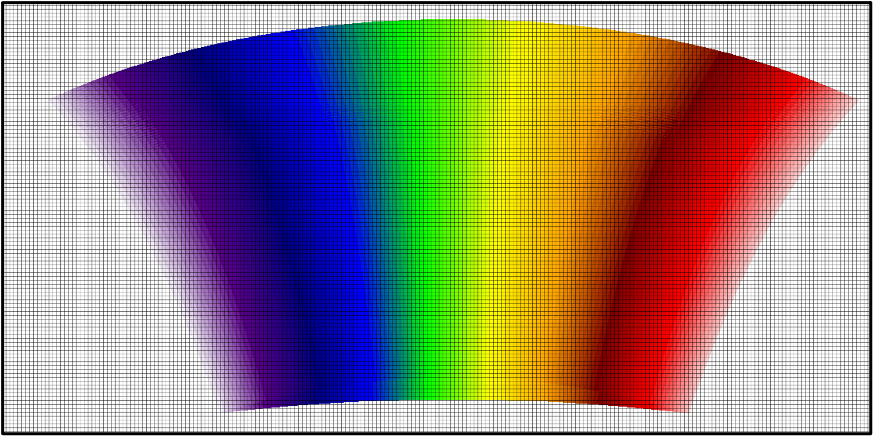
\includegraphics{Figures/附录/基础网格对兰伯特投影的等效描述示意图.png}
\caption{基础网格对兰伯特投影的等效描述示意图}
\label{fig:兰伯特投影的等效描述示意图}
\end{figure}
}

在模式框架章节中已经说明,CoLM的实际计算在patch层级进行,而patch的划分、数据生成则依赖于每个兰伯特投影网格element,因此在数据准备阶段需要考虑的是如何描述每个element的范围。在实现与CoLM的耦合中,匹配兰伯特投影的关键是将兰伯特投影的网格点的位置和范围与CoLM对应。实现方法是通过模式框架章节中介绍的使用多边形非结构网格来描述每一个兰伯特投影网格。具体地,在非结构网格CoLM的准备工作中涉及一个描述网格分配的Mesh网格。Mesh网格以极高分辨率对全球进行等经纬度划分(约1km网格,取决于陆面基础数据集的分辨率),通过对不同网格的染色区分出element。因此,如需实现对兰伯特投影的描述,只需将已有的区域模型投影网格根据其投影斑块的形状给Mesh上的对应细网格赋值即可实现用Mesh描述兰伯特投影的实际网格。如图~\ref{fig:兰伯特投影的等效描述示意图}~所示,兰伯特投影的每一个网格可以被若干个细网格Mesh等效的表示。兰伯特投影网格在等经纬度的投影上是曲线围成的小区域。而细网格Mesh以锯齿状的分布来模拟投影曲线,这存在理论上的误差。但是由于Mesh的细网格是基于当前最高分辨率的陆面基础数据(全球1公里,部分区域可达90m)构建的,采用平滑度更高的曲线进行拟合对模拟精度带来的改进将非常有限。至此,生成的Mesh网格即被用于地表资料的准备和后续计算,其流程可参考非结构网格CoLM的运行。非结构网格的CoLM可以稳定运行在目标网格后即可进行进一步耦合配置。

2. 计算流与时间管理

CPL7通过ESMF Clock特性作为主时钟进行时钟管理,而CoLM内部则通过更加直接的“年份+ Julian日+秒”的方式显式地管理积分时钟。因此实现时钟的统一,只需要在每次调用CoLM之前使用ESMF库的\texttt{ESMF\_ClockGet}函数获取耦合器当前时钟,再使用\texttt{ESMF\_TimeGet}将当前时钟转换为当前的显式日期(YYYY-MM-DD HH:MM:SS),接着,将获得的显式日期通过简单的计算换算成(YYYY JulianDay Second)的形式,传入CoLM的当前积分步时间即可。

每一次CoLM的运行既可以包含一个积分步也可运行多个积分步。在与CWRF模型耦合时,耦合频率和积分步长均设置为10分钟,即耦合器控制每10分钟调用一次CoLM,每次运行一个积分步。耦合框架也支持间隔更长的耦合频率,使得每次调用CoLM时完成多个积分步。使用CPL7耦合CoLM的时间循环流程见图~\ref{fig:CoLM的时间循环流程}。

{
\begin{figure}[htbp]
\centering
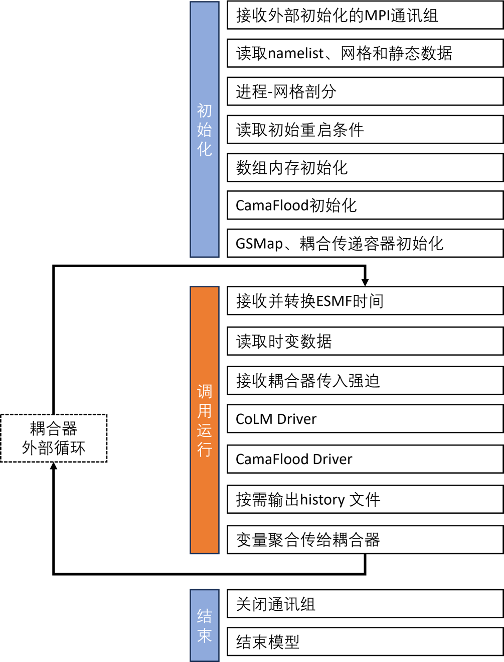
\includegraphics{Figures/附录/使用CPL7耦合CoLM的时间循环流程图.png}
\caption{使用CPL7耦合CoLM的时间循环流程图}
\label{fig:CoLM的时间循环流程}
\end{figure}
}

3. 进程-网格剖分

耦合系统中的不同分量与耦合器之间的数据交换的前提是描述各分量网格以及明确对应进程所负责的网格序号。CPL7-MCT提供了统一的数据类型GSMap(GlobalSegmentMap)来描述不同网格的剖分方式。对于非结构网格的CoLM来说,描述它的GSMap需要在每一个进程上进行初始化。当前版本CoLM相较过往版本设置了三种不同角色的进程,由于不同角色进程的内存数据存在很大差异,因此需要妥善管理。

初始化GSMap需要提取每个进程所负责的elemindex。一方面,master和io由于并不负责计算所以并不存储elemindex,因此初始化GSMap时必须置0。另一方面,耦合器所关注的强迫数据的分发和运行结果收集均只与worker进程有关,由于这些数据的传递仅发生在内存间网络通讯,不涉及外部文件IO,因此不需要额外经由IO进程中继,均直接通过worker进程与耦合器产生关联。因此,CoLM的GSMap初始化需要在worker上设置为各个element段的开始序号和长度,而在master和IO上设置为序号0长度0。

{
\begin{figure}[htbp]
\centering
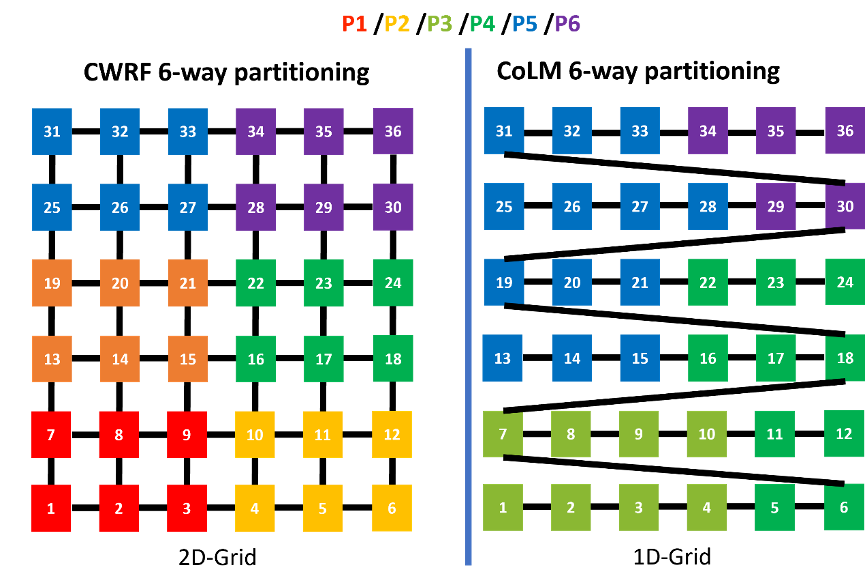
\includegraphics{Figures/附录/CWRF和非结构网格CoLM进程-网格剖分示意图.png}
\caption{CWRF和非结构网格CoLM进程-网格剖分示意图}
\label{fig:进程-网格剖分示意图}
\end{figure}
}

图~\ref{fig:进程-网格剖分示意图}~对比了CWRF和CoLM的网格剖分实例。假设此时两个模型均有36个网格需要剖分到6个进程上,结构网格CWRF和类似的2D网格仅需近似地分割为若干小矩形,在描述时每个进程标注网格开始序号和长度。对于非结构网格的CoLM,则对一维数组进行剖分。由于CoLM的master和IO进程不负责直接计算不能参与剖分,因此实际的网格-进程分配从第3进程开始,前两个进程的开始网格和分段长度均为0,如表~\ref{tab:CoLM剖分}所示。

\begin{table}[htbp]
\centering
\caption{非结构网格CoLM的GSMap分割示例}
\label{tab:CoLM剖分}
\begin{tabular}{@{}lccccccccccccc@{}}
\toprule
start  & 0 & 1 & 5 & 7 & 11 & 13 & 16 & 19 & 22 & 25 & 29 & 31 & 34 \\ \midrule
length & 0 & 4 & 2 & 4 & 2 & 3 & 3 & 3 & 3 & 4 & 2 & 3 & 3 \\ \midrule
pe\_loc & 1/2 & 3 & 4 & 3 & 4 & 5 & 4 & 5 & 4 & 5 & 6 & 5 & 6 \\ \bottomrule
\end{tabular}
\end{table}
